%% !TEX root = ../Thesis.tex
%% !TEX output_directory
\documentclass[11pt,a4paper,english,greek,twoside]{../Thesis}




\begin{document}
\chapter{Πειράματα και Αποτελέσματα Αναγνώρισης Δράσεων}
Έχοντας αναλύσει την εξαγωγή των χαρακτηριστικών από τα διαφορετικά κανάλια πληροφορίας, φτάνουμε στο σημείο της σύμμειξης των καναλιών προκειμένου να προκύψει μια ενιαία αναπαράσταση, κατάλληλη για ταξινόμηση. Αναζητούμε ένα συνδυασμό απόδοσης και επίδοσης, γνωρίζοντας ότι πιθανόν οι δύο αυτοί παράγοντες να είναι αντιμαχόμενοι. Στο κεφάλαιο αυτό θα εξετάσουμε θα εξετάσουμε την ταξινόμηση των εξαγόμενων χαρακτηριστικών των τμημάτων βίντεο με αρκετές διαφορετικές μεθόδους, συγκρίνοντας τα αποτελέσματά τους και τελικά ανάγοντας τη σύγκριση με άλλες μεθόδους της παγκόσμιας βιβλιογραφίας. Το πρόβλημα της ταξινόμησης γενικά, στην επιβλεπόμενη μάθηση, ορίζεται ως η εύρεση συνάρτησης βέλτιστης απεικόνισης νέων δεδομένων σε κάποια ή κάποιες από τις γνωστές κατηγορίες, έχοντας προηγηθεί εκπαίδευση του συστήματος με δεδομένα των οποίων οι ετικέτες είναι γνωστές. Αρχικά θα παρουσιάσουμε συνοπτικά τη φιλοσοφία της μεθόδου ταξινόμησης με χρήση Μηχανών Διανυσμάτων Υποστήριξης (SVM) και στη συνέχεια θα δούμε τις διάφορες μεθόδους που χρησιμοποιήσαμε κατά την ταξινόμηση, πρώτα θεωρητικά κι έπειτα πειραματικά.


\section{Θεωρητικό Υπόβαθρο}
\subsection{Μηχανές Διανυσμάτων Υποστήριξης (SVM)}
Οι Μηχανές Διανυσμάτων Υποστήριξης (στο εξής SVM, από τον αγγλικό όρο Support Vector Machine) είναι γενικευμένα, μη πιθανοτικά, γραμμικά μοντέλα ταξινομητών επιβλεπόμενης μάθησης. Ο αλγόριθμος SVM εισήχθησε στο \cite{cortes_1995} ως Δίκτυο Διανυμάτων Υποστήριξης. Ο στόχος του αλγορίθμου SVM είναι ο διαχωρισμός, με βάση τα δείγματα εκπαίδευσης, του χώρου χαρακτηριστικών σε υποχώρους με τρόπο τέτοιο ώστε να μεγιστοποιείται η απόσταση μεταξύ των υποχώρων διαφορετικών κλάσεων. Η ταξινόμηση γίνεται σύμφωνα με τον χώρο στον οποίο εμπίπτουν τα νέα δείγματα, οπότε ο αλγόριθμος SVM εκτελείται σε γραμμικό χρόνο, αφού αρκεί να υπολογισθεί ένα εσωτερικό γινόμενο των βαρών των χαρακτηριστικών, τα οποία βάρη προβάλλουν το διάνυσμα προς ανίχνευση στον κατάλληλλο υποχώρο, με το ίδιο το διάνυσμα προς ταξινόμηση. Επομένως, η εκπαίδευση ανάγεται σε ένα πρόβλημα βελτιστοποίησης, το οποίο γεωμετρικά ισοδυναμεί με τον βελτιστο διαχωρισμό του χώρου χαρακτηριστικών με χρήση υπερεπιπέδων. Το αντικείμενο είναι πλούσιο σε χρήση μαθηματικών εργαλείων, η αναφορά των οποίων ξεφεύγει από τον σκοπό αυτής της εργασίας. Παραπέμπουμε τον ενδιαφερόμενο στην παγκόσμια βιβλιογραφία, εκκινώντας από την αυθεντική εργασία \cite{cortes_1995}. Θα εξετάσουμε όμως εδώ τις διάφορες παραλλαγές που θα χρησιμεύσουν στην πορεία της εργασίας μας.

\begin{figure}
  \centering
  \noindent\makebox[\textwidth]{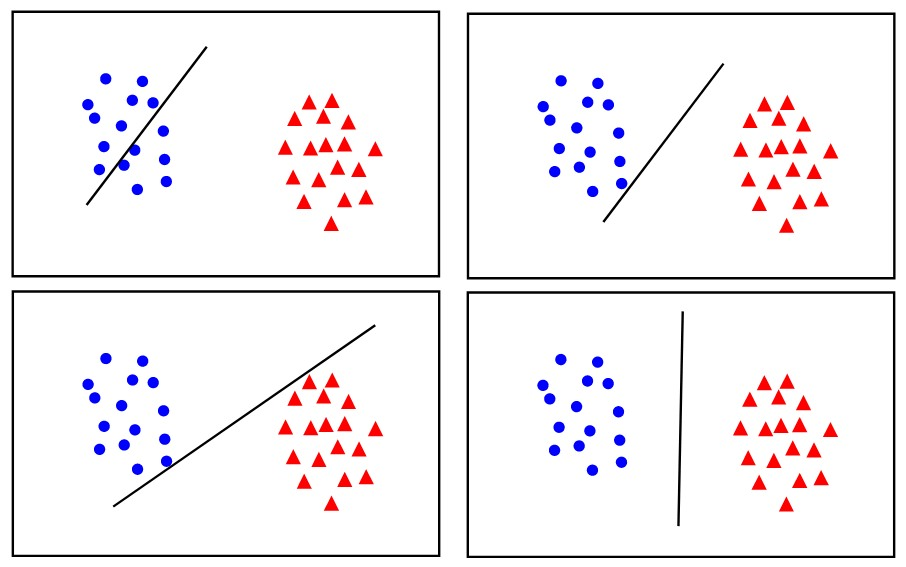
\includegraphics[scale=0.4]{{Images/chap6Separ}.jpg}}
  \caption{Είναι φανερό ότι σε ένα πρόβλημα ταξινόμησης δύο γραμμικά διαχωρίσιμων κλάσεων υπάρχουν άπειρες λύσεις. Ποια από αυτές είναι η προτιμότερη; Αν το κριτήριο είναι η ικανότητα γενίκευσης, τότε βέλτιστη λύση, για τα υπάρχοντα δεδομένα, είναι η γραμμή που αφήνει μέγιστο περιθώριο και για τις δύο κλάσεις, έτσι ώστε να διατηρείται ισορροπία μεταξύ των χώρων σφαλμάτων των κλάσεων. Ο αλγόριθμος SVM αναζητά τη βέλτιστη αυτή γραμμή, μέσα από ένα πρόβλημα ελαχιστοποίησης κόστους. Η αναζήτηση βέλτιστης λύσης και όχι απλά λύσης διαχωρίζει τον ταξινομητή SVM από τους υπόλοιπους γραμμικούς ταξινομητές. Εικόνα από \cite{scikit_2011}}
  \label{fig:chap6Separ}
\end{figure}

\subsubsection{Μη Γραμμική SVM: Το Τέχνασμα Πυρήνα}
Από τον ορισμό του, ο αλγόριθμος SVM είναι γραμμικός, οπότε δε λειτουργεί ικανοποιητικά για μη γραμμικά διαχωρίσιμες κλάσεις. Ωστόσο, συχνά χρησιμοποιείται μια παραλλαγή του αλγορίθμου, καθιστώντας τον επαρκή και για μη γραμμικά προβλήματα. Στην πράξη, μετασχηματίζουμε τον χώρο χαρακτηριστικών σε έναν άλλο χώρο, συνήθως μεγαλύτερης διάστασης, στον οποίο τα χαρακτηριστικά αποκτούν ιδιότητες γραμμικής διαχωρισιμότητας. Η ταξινόμηση γίνεται στον νεο αυτό χώρο, οπότε κατά τη φάση εκπαίδευσης, κάθε δείγματα υφίσταται μια μη γραμμική απεικόνιση και το πρόβλημα βελτιστοποίησης ανάγεται σε εύρεση των υπερεπιπέδων που διαχωρίζουν βέλτιστα τις περιοχές αυτού του νέου χώρου. Αν ωστόσο μεταβούμε πίσω στον αρχικό χώρο χαρακτηριστικών, θα δούμε οτι τα υπερεπίπεδα έχουν λάβει μορφή υπερεπιφανειών, δίνοντας την εντύπωση του μη γραμμικού ταξινομητή. Η συνάρτηση μεταφοράς στον νέο υπερχώρο ονομάζεται συνάρτηση πυρήνα (kernel) και ως εκ τούτου η όλη διαδικασία αναφέρεται συχνά ως τέχνασμ πυρήνα (kernel trick) λόγω της ψευδαίσθησης της μη γραμμικότητας.

\begin{figure}
  \centering
  \noindent\makebox[\textwidth]{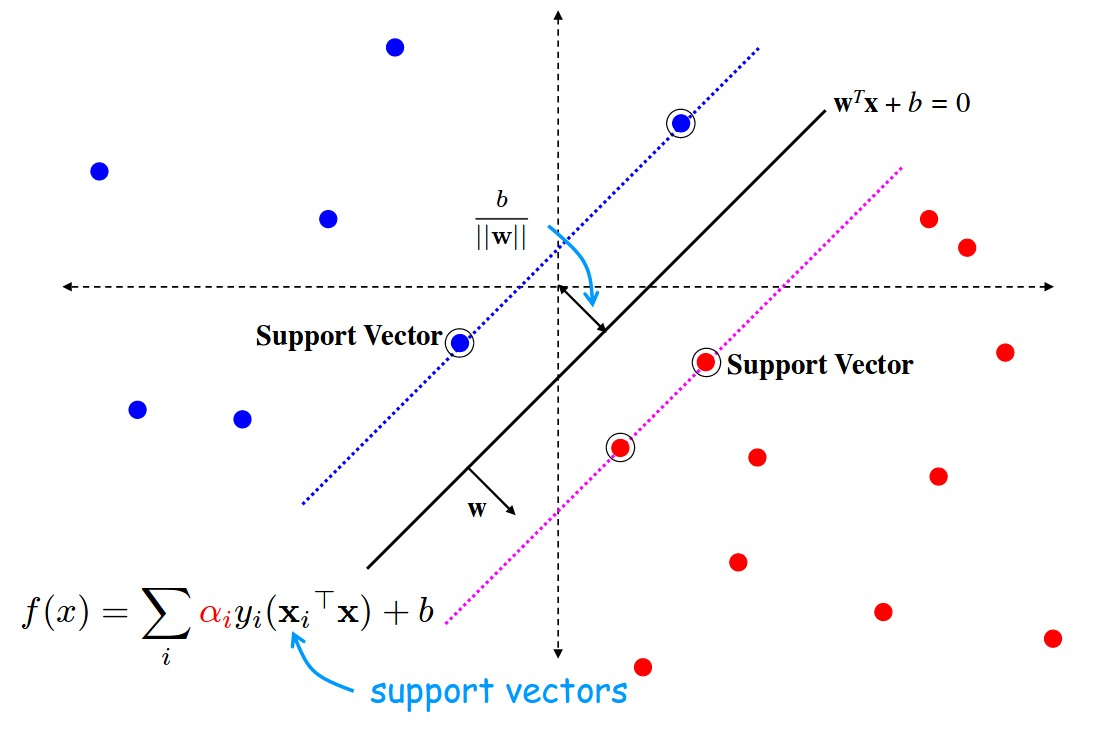
\includegraphics[scale=0.35]{{Images/chap6SVMSep}.jpg}}
  \caption{Η μέθοδος ταξινόμησης SVM αναζητά τους βέλτιστους εκπροσώπους των ορίων των κλάσεων, τα λεγόμενα Διανύσματα Υποστήριξης (Support Vectors). Σύμφωνα με αυτά τα διανύσματα, οριοθετεί γραμμικά τους χώρους των κλάσεων και λαμβάνει τη μεσοπαράλληλο των γραμμικών συνόρων ως τη βέλτιστη διαχωριστική γραμμή μεταξύ των κλάσεων. Σε παραπάνω διαστάσεις, η διαχωριστική επιφάνεια είναι ένα υπερεπίπεδο. Με μετασχηματισμό πυρήνα, το υπερεπίπεδο αυτό μπορεί να αναπαριστά μια υπερεπιφάνεια η οποία προκύπτει από μια μη γραμμική απεικόνιση του χώρου χαρακτηριστικών σε έναν άλλο, διαφορετικής πιθανόν διάστασης. Εικόνα από \cite{scikit_2011}}
  \label{fig:chap6SVMSep}
\end{figure}

\par Στη βιβλιογραφία έχουν αναφερθεί αρκετές συναρτήσεις πυρήνα. Κλασσική περίπτωση είναι αυτή του τετραγωνικού ή του πολυωνυμικού πυρήνα, που μεταφέρει τα δείγματα σε έναν χώρο όπου ένα πολυώνυμο θα απεικονιζόταν ως ευθεία (υπερεπίπεδο). Στην παρούσα εργασία χρησιμοποιούμε τον συνδυασμό χαρακτηριστικών με $\chi^{2}$ πυρήνα, οποίος βρέθηκε ότι συνδυάζεται γόνιμα με την προσέγγιση του Σάκου Λέξεων στην αναγνώριση τόσο εικόνων (αντικειμένων) όσο και βίντεο (δράσεων) \cite{laptev_2008}, \cite{wang_2011}. Η προσέγγιση η οποία ακολουθούμε σε αυτή τη συνεργασία είναι ίδια με του \cite{wang_2011} και στοχεύει στην από κοινού αναπαράσταση των διαφορετικών χαρακτηριστικών. Αν έχουμε $N$ διαφορετικά κανάλια χαρακτηριστικών, τότε η συνάρτηση πυρήνα περιγράφεται από τη σχέση:

\begin{equation}\label{eq:ChiSKernel}
    K(x_i,x_j)=exp\big(-\sum_{c=1}^{N} \frac{1}{A^{c}} D(x_{i}^{c},x_{j}^{c}) \big)
\end{equation}

όπου $D(x_{i}^{c},x_{j}^{c})$ είναι η $\chi^{2}$ του βίντεο $x_{i}$ από το βίντεο $x_{j}$ στα χαρακτηριστικά του καναλιού $c$. $A^{c}$ είναι η μέση τιμή $\chi^{2}$ αποστάσεων μεταξύ των δειγμάτων εκπαίδευσης στο κανάλι $c$. Η $\chi^{2}$ απόσταση δύο διανυσμάτων $x$ και $y$ δίνεται από την εξίσωση:

\begin{equation}\label{eq:ChiS}
    D(x,y)=exp \bigg(-\gamma \sum_{i} \frac{(x[i]-y[i])^{2}}{x[i]+y[i]} \bigg)
\end{equation}

Η προσέγγιση αυτή απεικονίζει κάθε δείγμα με ένα διάνυσμα πραγματικών αριθμών μήκους ίσο με τον αριθμό των δειγμάτων εκπαίδευσης. Η μέθοδος έχει αποδειχθεί εύρωστη στο συνδυασμό πολλαπλών καναλιών διαφορετικής πληροφορίας.

\begin{figure}
  \centering
  \noindent\makebox[\textwidth]{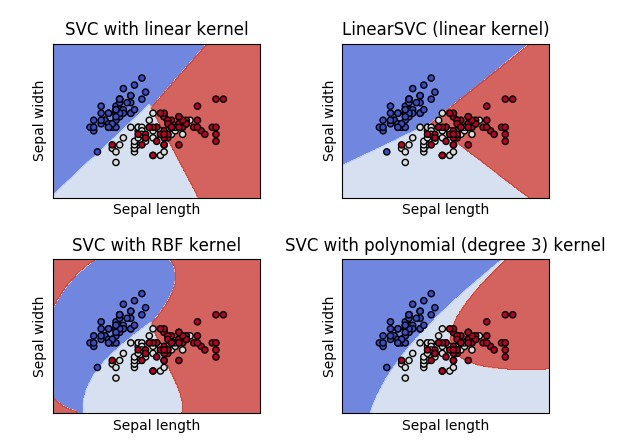
\includegraphics[scale=0.5]{{Images/chap6SVMScikit}.jpg}}
  \caption{Ο ίδιος χώρος δεδομένων μπορεί να διαχωριστεί αρκετά διαφορετικά αν μεσολαβήσει μη γραμμική απεικόνιση σε έναν άλλο χώρο όπου μια μη γραμμική διαχωριστική επιφάνεια μπορεί να γίνει διαχωριστική. Για παράδειγμα, σε έναν χώρο που προκύπτει από έναν πολυωνυμικό μετασχηματισμού βαθμού $n$, ένα πολυώνυμο βαθμού $n$ μπορεί να αναπαριστά μια ευθεία. Μετασχηματισμοί αυτού του είδους χρησιμοποιούνται για να διευκολύνουν τη γραμμική διαχωρισιμότητα και την αποδοτική χρήση της μεθόδου SVM. Εικόνα από \cite{scikit_2011}}
  \label{fig:chap6SVMScikit}
\end{figure}

\subsubsection{Πιθανοτική SVM: Η Μέθοδος Platt}
Οι μη πιθανοτικοί ταξινομητές επιστρέφουν την κατηγορία στην οποία τοποθετούν ένα δείγμα σύμφωνα με κάποια μετρική. Ωστόσο η μετρική αυτή δεν έχει φυσική ερμηνεία και μεταξύ των τιμών που λαμβάνει δε μπορεί να γίνει απευθείας σύγκριση. Από την άλλη, δε μας παρέχεται κάποιο μέτρο βεβαιότητας της ταξινόμησης έτσι ώστε να μπορεί να χρησιμοποιηθεί σε επόμενο στάδιο για κάποιο συνδυασμό με άλλους πιθανοτικούς ταξινομητές. Η λύση που προτάθηκε σε αυτό ήταν η πιθανοτική αντιστάθμιση (probability calibration). Πιο σχετική με την περίπτωση των SVM είναι η μέθοδος Κλιμάκωσης Platt (Platt Scaling) η οποία προτάθηκε στο \cite{platt_1999}. Η μέθοδος επιχειρεί να προσεγγίσει με μια εκθετική κατανομή πιθανοτήτων την πραγματική κατανομή πιθανοτήτων εξόδου, υπολογίζοντας παραμέτρους σύμφωνα με τα δείγματα εκπαίδευσης. Αν για παράδειγμα ο ταξινομητής κατατάσσει σε κατηγορίες το δείγμα $x$ βασιζόμενος σε μια υπολογισθείσα συνάρτηση $f(x)$, τότε η μέθοδος Platt εκτιμά μια κατανομή

\begin{equation}\label{eq:Platt}
    P(y|x)=\frac{1}{1+exp(Af(x)+b)}
\end{equation}

με τα $A$ και $b$ να αποτελούν δυο βαθμωτές παραμέτρους που μαθαίνονται κατά τη διάρκεια εκπαίδευσης.


\subsection{Το Σχήμα Tf-Idf}
Στην θεωρια πληροφορίας, το σχήμα Tf-Idf (Term frequency - Inverse document frequency) είναι μια αριθμητική στατιστική μετρική που αναδεικνύει τη σημασία μιας λέξης σε ένα κείμενο από μια συλλογή εγγράφων. Η τιμή της μετρικής αυτής αυξάνει ανάλογα με τον αριθμό των φορών που η λέξη εμφανίζεται μέσα στο κείμενο, αλλά η εμφάνιση αντισταθμίζεται από τη συχνότητα της λέξης στο σύνολο των κειμένων της συλλογής. Έτσι λαμβάνεται υπόψιν το γεγονός ότι κάποια λέξη μπορεί να είναι γενικού σκοπού και να εμφανίζεται σε πολλά κείμενα πολλές φορές, χωρίς αυτό να αποδίδει κατι ξεχωριστό στην εμφάνισή της. Το σχήμα Tf-Idf συνδυάζει τους δύο όρους Term frequency και Invese document frequency. Ο πρώτος όρος εισήχθη στο \cite{luhn_1957} και εκφράζει τον αριθμό των φορών που ένας όρος εμφανίζεται σε ένα κείμενο. Ο δεύτερος όρος εμφανίστηκε στο \cite{jones_1972} και πρόκειται για το αντίστροφο της συχνότητας εμφάνισης της λέξης στο σύνολο των κειμένων. Έστω λοιπόν $d$ ένα κείμενο από μια συλλογή κειμένων $D$ και $t$ μια λέξη. Τότε η μετρική Tf-Idf για την εμφάνιση της λέξης $t$ στο κείμενο $d$ έχει την έκφραση

\begin{equation}\label{eq:Tfidf}
    tfidf(t,d,D)=tf(t,d) \times idf(t,D)
\end{equation}

Η αναλυτική έκφραση του σχήματος ποικίλλει ανάλογα με τη χρήση ή τα δεδομένα. Πιο συνήθεις εκφράσεις οι $1+logf_{t,d}$ και $log(1+\frac{N}{n_t})$ οι οποίες στηρίζονται στο κομμάτι Tf και στο Idf αντίστοιχα.


\section{Η Δική Μας Προσέγγιση και Τα Πειραματικά αποτελέσματα}
\subsection{Οι Ρυθμίσεις του Συνόλου Δεδομένων}
Σε αυτό το σημείο παρουσιάζουμε τις ρυθμίσεις εκπαίδευσης και ελέγχου πάνω στο σύνολο δεδομένων MPII Cooking Activities. Το σύνολο περιέχει 44 βίντεο. Από αυτά, χρησιμοποιήσαμε τα 24 για εκπαίδευση, με τρόπο που να εξασφαλίζει την εμφάνιση όλων των κατηγοριών τόσο στα δεδομένα εκπαίδευσης όσο και στα δεδομένα ελέγχου. Παρότι το πλήθος των δράσεων είναι 65, επιλέγουμε τις 61 από αυτές, συσχετίζοντάς τες με τις εναπομείνασες 4 με δράσεις από το λεξιλόγιό μας. Οι επισημειώσεις αντικειμένων υπάρχουν στη νεότερη έκδοση του συνόλου δεδομένων. Από τις κατηγορίες αντικειμένων αυτές, κρατάμε μόνο τις 92, αφού μόνο αυτές εμφανίζονται στα βίντεο εκπαίδευσης και στα βίντεο ελέγχου. Λεπτομέρειες για τις παρεμβάσεις στο σύνολο δεδομένων αναφέρονται στο Παράρτημα \ref{dataset}. Παρά την ελαφρά τροποποίηση όσον αφορά το πλήθος των δράσεων προς αναγνώριση, τα πειράματα δείχνουν να συμφωνούν ως προς τα αποτελέσματα, με την αυθεντική υλοποίηση των \cite{rohrbach_2012}, την οποία και υλοποιήσαμε ξανά.

\par Για όλα τα πειράματα ταξινόμησης έγινε μελέτη πάνω σε ποικιλία ταξινομητών και αλγορίθμων. Τελικά, επιλέχθηκε ο ταξινομητής SVM καθώς συνδυάζει υψηλή απόδοση και επίδοση. Οι παράμετροι του ταξινομητή επιλέχθηκαν με cross-validation ξεχωριστά για κάθε πείραμα. Η μετρική σε όλα τα πειράματα είναι η σταθμισμένη Mean Average Precision (mAP), η οποία χρησιμοποιήθηκε από την πρώτη εργασία πάνω στο συγκεκριμένο σύνολο δεδομένων \cite{rohrbach_2012} και έκτοτε παραμένει ως μετρική για ενιαία σύγκριση αποτελεσμάτων στο σύνολο αυτό. Η μετρική Precision ορίζεται από την εξίσωση:

\begin{equation}\label{eq:Precision}
    Precision=\frac{|\{True Positives\}|}{|\{Predicted Positives\}|}
\end{equation}

Διαισθητικά, η μετρική Precision εξετάζει το κατά πόσο ένα σύστημα είναι ικανό να απορρίπτει τα αρνητικά δείγματα. Είναι φανερό ότι υψηλή τιμή Precision δεν εξασφαλίζει ακριβή ταξινόμηση. Επίσης είναι φανερό ότι η μετρική είναι ορισμένη για το πρόβλημα δύο κλάσεων. Θα δούμε τη γενίκευση στην περίπτωση των πολλών κλάσεων αφού ορίσουμε την ποσότητα Average Precision (AP) ως εξής:

\begin{equation}\label{eq:APrecision}
    Average Precision=\int_0^{1} p(r)dr
\end{equation}N
Τώρα μπορούμε να λάβουμε τον σταθμισμένο μέσο των τιμών AP για κάθε κλάση (θεωρώντας $N$ δυαδικά προβλήματα, με $N$ το πλήθος των κλάσεων) για να εκφράσουμε μια μετρική κατάλληλη για το πρόβλημα πολλών κλάσεων ως εξής:

\begin{equation}\label{eq:mAP}
    \text{weighted mAP}=\frac{\sum_{i=1}^{N}w_iAP[i]}{\sum_{i=1}^{N} w_i}
\end{equation}


\subsection{Αξιοποίηση Πληροφορίας Όρασης Χαμηλού Επιπέδου}
Σε πρώτη φάση επιχειρούμε να δούμε τη δύναμη των οπτικών χαρακτηριστικών. Η πληροφορία αυτή κωδικοποιεί την κίνηση και μπορεί να εξασφαλίσει ότι μια κίνηση συμβαίνει, σε αντίθεση με τη σημασιολογία που δεν μπορεί να εγγυηθεί κάτι τέτοιο. Ελέγχουμε διαφορετικούς τρόπους συνδυασμού των χαρακτηριστικών. Ο πρώτος είναι και ο προτεινόμενος από την αυθεντική εργασία των Πυκνών Τροχιών και του \cite{rohrbach_2012} και κάνει χρήση του πυρήνα $\chi^2$ ώστε να συνδυάσει τα κανονικοποιημένα (ώστε να αθροίζουν στη μονάδα) ιστογράμματα για τους έξι τύπους οπτικών χαρακτηριστικών. Τα δείγματα εκπαίδευσης είναι 2888, οπότε και η διάσταση του διανύσματος που προκύπτει από αυτό τον μετασχηματισμό είναι 2888. Ένα τέτοιο διάνυσμα περιέχει την οπτική πληροφορία ενός τμήματος βίντεο. Μια άλλη μέθοδος συνδυασμού είναι η κωδικοποίηση των διανυσμάτων με το σχήμα Tf-Idf και η παράθεσή τους (concatenation). Το προκύπτον διάνυσμα έχει μήκος $4 \times 4000 + 3336 + 1536=20872$, τιμή η οποία επιβραδύνει αλλά δεν δυσχεραίνει τη μέθοδο SVM στην απόδοση, καθώς ο αλγόριθμος μπορεί να λειτουργεί ικανοποιητικά σε διαστάσεις πολύ μεγαλύτερες από το πλήθος των δειγμάτων εκπαίδευσης. Τέλος, συνδυάζουμε τις παραπάνω μεθόδους, πρώτα μεταχηματίζοντας κατά Tf-Idf και μετά εφαρμόζοντας τον μη γραμμικό πυρήνα. Τα αποτελέσματα φαίνονται εδώ:

\begin{table}[H]
	\centering
    \begin{tabular}{| l | l | l | l |}
    \hline
    \textbf{Method} & \textbf{mAP} \\ \hline
    Original method with $\chi^2$ kernels (\cite{rohrbach_2012}) & 57.9 \\ \hline
    \textbf{Original method with $\chi^2$ kernels (ours)} & \textbf{58.4} \\ \hline
    Tf-Idf features stacked method & 51.88 \\ \hline
    Tf-Idf combined with Chi-Squared kernels & 58.27 \\
    \hline
    \end{tabular}
	\label{tab:LLVSResults}
	\caption{Αποτελέσματα των μεθόδων που αξιοποιούν μόνο πληροφορία χαμηλού επιπέδου Όρασης Υπολογιστών. Η προτεινόμενη μέθοδος φαίνεται ότι υπερισχύει των υπολοίπων και ότι η χρήση $\chi^2$ πυρήνα είναι απαραίτητη.}
\end{table}

\par Καταρχάς, στον πίνακα παρουσιάσαμε, πέραν των τριών δικών μας αποτελεσμάτων, το αποτέλεσμα του \cite{rohrbach_2012}. Ο λόγος είναι η σύγκριση της δικής μας υλοποίησης με τη δική τους, του ίδιου αλγορίθμου, αλλά με 61 κατηγορίες αντί για 65. Βλέπουμε ότι αφαιρώντας 4 κατηγορίες αποκτούμε μικρό προβάδισμα, όμως γενικά το αποτέλεσμα δεν αλλοιώνεται σημαντικά και έτσι τα αποτελέσματα της εργασίας μας παραμένουν συγκρίσιμα με αυτά της παγκόσμιας βιβλιογραφίας. Τώρα συγκρίνοντας τις τρεις δικές μας υλοποιήσεις, βλέπουμε ότι η κωδικοποίηση Tf-Idf είναι πολύ πιο ασθενής από την μετατροπή των χαρακτηριστικών με $\chi^2$ πυρήνες. Ο συνδυασμός τους είναι ελάχιστα λιγότερο ισχυρός από τη μέθοδο $\chi^2$ πυρήνων μόνη της, δείχνοντας ότι η χρήση αυτού του μετασχηματισμού εμπεριέχει την πιο επαρκή αναπαραστική δύναμη. Θα δούμε στη συνέχεια ωστόσο ότι αυτό ανατρέπεται όταν εισάγονται επιπλέον χαρακτηριστικά.

\subsection{Αξιοποίηση Σημασιολογικής Πληροφορίας: Αντικείμενα}
Στη συνέχεια εισάγουμε την σημασιολογική πληροφορία των αντικειμένων. Η πληροφορία αυτή εμπεριέχει τη σχέση δράσεων και αντικειμένων, εξασφαλίζοντας ότι μια σχέση πραγματοποιείται. Εξετάζουμε 6 τρόπους συνδυασμού χαρακτηριστικών. Οι πρώτοι τρεις χρησιμοποιούν τον συνδυασμό Tf-Idf και $\chi^2$ πυρήνων για την αναπαράσταση των οπτικών χαρακτηριστικών, οπότε η διάσταση αυτού του τμήματος πληροφορίας είναι 2888. Για τα ιστογράμματα αντικειμένων δοκιμάζουμε απλή συνένωση, μετασχηματισμό Tf-Idf και συνένωση και μετασχηματισμό Tf-Idf και συμπερίληψη στον πυρήνα $\chi^2$ ως έβδομο κανάλι πληροφορίας. Ως αποτέλεσμα, η διάσταση του διανύσματος ενός τμήματος βίντεο είναι 2980 (ως 2888+92) για τις δύο πρώτες περιπτώσεις και 2888 για την τρίτη. Πέραν αυτών των συνδυασμών, δοκιμάζουμε μετατροπή $\chi^2$ πυρήνα για τα οπτικά χαρακτηριστικά (χωρίς Tf-Idf) και απλή συνένωση (τελική διάσταση 2980) ή συμπερίληψη στον πυρήνα ως έβδομο κανάλι (τελική διάσταση 2888) για τα ιστογράμματα αντικειμένων. Τέλος, μια ακόμα μέθοδος συνδυασμού είναι η συνένωση των οπτικών χαρακτηριστικών αφού προηγηθεί κωδικοποίηση με το σχήμα Tf-Idf και έπειτα συνένωση με τα ιστογράμματα αντικειμένων, οδηγώντας σε μια διάσταση 20964. Σε όλες τις μεθόδους χρησιμοποιήθηκαν οι ίδιες επισημειώσεις αντικειμένων, οι οποίες λαμβάνονται από το συγγενικό σύνολο δεδομένων MPII Cooking 2. Για να μοντελοποιήσουμε τον θόρυβο από την ανίχνευση αντικειμένων, εισάγουμε τεχνητά θόρυβο στα δείγματα εκπαίδευσης για τις περιπτώσεις όπου για ένα τμήμα οι επισημειώσεις δείχνουν ότι δεν υπάρχουν αντικείμενα. Ο θόρυβος αφορά 1, 2, 3 ή 4 τυχαία αντικείμενα τα οποία εισάγονται με πιθανότητα 0.15 για την κάθε περίπτωση, ενώ με πιθανότητα 0.4 αφήνουμε το διάνυσμα χωρίς θόρυβο. Στον πίνακα συγκρίνουμε τα αποτελέσματα αυτών των τεχνικών:

\begin{table}[H]
	\centering
    \begin{tabular}{| l | l | l | l |}
    \hline
    \textbf{Method} & \textbf{mAP} \\ \hline
    $\chi^2$ LLV features combined with objects & 65.1 \\ \hline
    $\chi^2$ LLV features and $\chi^2$ Tf-Idf objects & 58.33 \\ \hline
    $\chi^2$ Tf-Idf LLV features, combined with objects & 64.8 \\ \hline
    $\chi^2$ Tf-Idf LLV features and Tf-Idf objects & 62.86 \\ \hline
    $\chi^2$ Tf-Idf LLV features and $\chi^2$ Tf-Idf objects  & 54.76 \\ \hline
    \textbf{Stacked Tf-Idf LLV features combined with objects} & \textbf{65.74} \\
    \hline
    \end{tabular}
	\label{tab:SemResults}
	\caption{Αποτελέσματα των μεθόδων που αξιοποιούν και πληροφορία αντικειμένων σε σύγκριση. Βλέπουμε ότι τα ποσοστά ανεβήκαν και ότι η ανάγκη για $\chi^2$ μετασχηματισμό υποχωρεί.}
\end{table}

\par Πρώτη παρατήρηση είναι σίγουρα η ενίσχυση των αποτελεσμάτων κατά πολύ μεγάλο περιθώριο κέρδους. Η συμπληρωματικότητα των καναλιών οπτικής και σημασιολογικής πληροφορίας γίνεται φανερή και πειραματικά. Μάλιστα, έχει ενδιαφέρον η παρατήρηση ότι ο συνδυασμός των καναλιών εμπλουτίζει τόσο τη διακριτική ικανότητα που δεν είναι απαραίτητος ο μετασχηματισμός με $\chi^2$ πυρήνες για τα οπτικά χαρακτηριστικά. Για το τμήμα αντικειμένων, η πιο αξιέπαινη αναπαραστατική δύναμη εμφανίζεται με την απλή συνένωση, χωρίς επιπλέον μετασχηματισμούς. Τέλος, βλέπουμε ότι εισάγοντας την πληροφορία αντικειμένων, το σχήμα Tf-Idf μπορεί να ξεπεράσει την απόδοση του $\chi^2$ μετασχηματισμού για τα οπτικά χαρακτηριστικά. Αυτή είναι μια ιδιαίτερα σημαντική παρατήρηση και από άποψη επίδοσης, καθώς ο $\chi^2$ μετασχηματισμός είναι αρκετά δαπανηρός σε σχέση με το σχήμα Tf-Idf.

\subsection{Αξιοποίηση Σημασιολογικής Πληροφορίας: Τύποι Λαβής}
Η τελευταία μορφή πληροφορίας που εισάγουμε είναι αυτή των τύπων λαβής (grasping types). Το κανάλι αυτό εμπεριέχει το χειρισμό των αντικειμένων και το σχηματισμό των χεριών. Δοκιμάζουμε την απευθείας συνένωση των ιστογραμμάτων τύπων λαβής και αντικειμένων με τα κατά $\chi^2$ μετασχηματισμένα, τα κατά Tf-Idf μετασχηματισμένα και σωρρευμένα και τα απλώς σωρρευμένα οπτικά χαρακτηριστικά, οδηγώντας σε διαστάσεις 2990, 20974 και 20974 αντίστοιχα. Τα αποτελέσματα φαίνονται συγκριτικά στον πίνακα:

\begin{table}[H]
	\centering
    \begin{tabular}{| l | l | l | l |}
    \hline
    \textbf{Method} & \textbf{mAP} \\ \hline
    $\chi^2$ LLV features combined with objects and grasping & 65.15 \\ \hline
    \textbf{Stacked Tf-Idf LLV features combined with objects and grasping} & \textbf{66.45} \\ \hline
    Stacked LLV features combined with objects and grasping & 66.25 \\
    \hline
    \end{tabular}
	\label{tab:GraspResults}
	\caption{Αποτελέσματα των μεθόδων που αξιοποιούν και πληροφορία τύπων λαβής. Υπάρχει μικρή βελτίωση στην απόδοση, ενώ η ανάγκη για $\chi^2$ μετασχηματισμό εξαλείφεται.}
\end{table}

\par Από τον παραπάνω πίνακα μπορούμε να εξάγουμε πολλά χρήσιμα συμπεράσματα. Καταρχάς, η εισαγωγή πληροφορίας για τον τύπο λαβής υποβοηθά την ταξινόμηση, έστω κατά ένα μικρό περιθώριο κέρδους, το οποίο είναι αναμενόμενο λόγω της απουσίας επισημειώσεων για χέρια και τύπους λαβής στο σύνολο δεδομένων. Η αύξηση της απόδοσης είναι μεγαλύτερη στην περίπτωση του συνδυασμού με κατά Tf-Idf μετασχηματισμένα οπτικά χαρακτηριστικά, δείχνοντας ότι ο $\chi^2$ μετασχηματισμός μπορεί να οδηγήσει σε κόρο την απόδοση, χωρίς όμως να έχουμε επαρκείς αποδείξεις για αυτό. Η κωδικοποίηση με το σχήμα Tf-Idf μπορεί επομένως να αντικαταστήσει τον $\chi^2$ μετασχηματισμό σε αυτούς τους συνδυασμούς. Από την άλλη, μικρή διαφορά υπάρχει και από την απλή συνένωση, η οποία είναι φανερά πιο αποδοτική χρονικά.


\subsection{Επανεκτίμηση Πιθανοτήτων Εξόδου}
Στο κεφάλαιο 2 προβήκαμε στην υπόθεση ότι αντικείμενα και χαρακτηριστικά χαμηλού-επιπέδου όρασης εμφανίζονται ανεξάρτητα, άρα

\begin{equation}\label{eq:c6Probs}
    P(\alpha | vocabulary, features)=P(\alpha|vocabulary) \times P(\alpha|features)
\end{equation}

Ήρθε επομένως η ώρα να ελέγξουμε την καρποφορία αυτής της επιλογής. Εκπαιδεύουμε τρεις ταξινομητές SVM με εκτίμηση πιθανοτήτων μέσω Κλιμάκωσης Platt. Για τον πρώτο ταξινομητή συνενώνουμε ιστογράμματα αντικειμένων με κατά Tf-Idf μετασχηματισμένα ιστογράμματα οπτικών χαρακτηριστικών. Προσθέτουμε στα παραπάνω και τα ιστογράμματα τύπων λαβής για να εκπαιδεύσουμε τον δεύτερο ταξινομητή. Ο τελευταίος ταξινομητής εκπαιδεύεται πάνω στη σώρρευση μη μετασχηματισμένων ιστογραμμάτων οπτικών χαρακτηριστικών, αντικειμένων και τύπων λαβής. Από τους ταξινομητές αυτούς λαμβάνουμε την κατανομή $P(\alpha|features)$. Στηριζόμαστε στα ιστογράμματα αντικειμένων που ανιχνεύθησαν για να εξάγουμε την κατανομή $P(\alpha|vocabulary)$. Στην προκειμένη, ο όρος $vocabulary$ αφορά μόνο τα αντικείμενα. Η διαφοροποίηση έγκειται στο ότι η κατανομή αυτή εξάγεται από πληροφορία κειμένου, οπότε στην πράξη πρόκειται για έναν συνδυασμό διαφορετικών καναλιών πληροφορίας.

\par Το σύνολο δεδομένων MPII Cooking 2, που αποτελεί συνέχεια, όπως έχουμε αναφέρει, του MPII Cooking Activies, περιέχει σύνολο περιγραφών για τα βίντεο και τις δράσεις τους. Το σύνολο περιγραφών έχει γραφεί σε φυσική γλώσσα και χρησιμοποιεί τις λέξεις του λεξιλογίου μας, οπότε μπορεί να χρησιμεύσει για την εξαγωγή των σχέσεων δράσεων-αντικειμένων. Από τα κείμενα αυτά εξάγονται οι επισημειώσεις ιστογραμμάτων αντικειμένων. Ουσιαστικά, η χρήση των λεξεων του λεξιλογίου στην ίδια κύρια πρόταση αυξάνει την πιθανότητα συσχέτισής τους. Για κάθε δράση μετράμε τη σχετική συχνότητα συνδυασμού της με κάθε λέξη του λεξιλογίου μας (ως προς τα αντικείμενα) και ορίζουμε αυτή ως πιθανότητα της δράσης δεδομένης της εμφάνισης της λέξης. Επειδή υπάρχουν δράσεις που δεν έχουν συνδυαστεί με όλα τα αντικείμενα, εφαρμόζουμε ομαλοποίηση κατά Laplace στην φάση εξαγωγής των σχετικών συχνοτήτων, οι οποίες τώρα θα δίνονται από τη σχέση

\begin{equation}\label{eq:c6Probs2}
    P(\alpha | object_i)=\frac{T_{\alpha,i}+1}{\sum_{i \in Objects} (T_{\alpha,i}+1)}
\end{equation}

δηλαδή προσθέτουμε 1 στις εμφανίσεις κάθε αντικειμένου μαζί με τη δράση $\alpha$. Έτσι αποφεύγουμε να γενικεύσουμε τη μηδενική πιθανότητα εμφάνισης λόγω πιθανώς περιορισμένου συνόλου θετικών δειγμάτων. Κατά τη φάση ελέγχου, εφαρμόζουμε τη σχέση \ref{eq:c6Probs} θεωρώντας ως $vocabulary$ τα αντικείμενα τα οποία εμφανίστηκαν. Δεν συμπεριλαμβάνουμε τη μη εμφάνιση στον υπολογισμό των πιθανοτήτων καθώς πειραματικά διαπιστώσαμε ότι δεν προσφέρει πολλά. Τρέξαμε τα πειράματα για τους 3 ταξινομητές χρησιμοποιώντας τα υπολογισμένα αλλά και τα πραγματικά αντικείμενα (επισημειώσεις) ώστε να εξαντλήσουμε τα οφέλη αυτών των τεχνικών. Τα αποτελέσματα φαίνονται στον πίνακα:

\begin{table}[H]
	\centering
    \begin{tabular}{| l | l | l | l |}
    \hline
    \textbf{Method} & \textbf{mAP} \\ \hline
    Stacked Tf-Idf LLV features combined with objects & 66.43 \\ \hline
    Stacked Tf-Idf LLV features combined with GT objects & 73.11 \\ \hline
    Stacked Tf-Idf LLV features combined with objects and grasping & 67.1 \\ \hline
    Stacked Tf-Idf LLV features combined with GT objects and grasping & 73.17 \\ \hline
    Stacked LLV features combined with objects and grasping & 67.25 \\ \hline
    \textbf{Stacked LLV features combined with GT objects and grasping} & \textbf{73.4} \\
    \hline
    \end{tabular}
	\label{tab:TuningResults}
	\caption{Αποτελέσματα των μεθόδων που προσαρμόζουν τις πιθανότητες στην έξοδο. Η υπόθεση στατιστικής ανεξαρτησίας των δύο καναλιών, οπτικής και γλωσσικής πληροφορίας ενσωματώνει σημασιολογία υψηλότερου επιπέδου η οποία συνεισφέρει σημαντικά στην αποτελεσματική ταξινόμηση.}
\end{table}

Όπως γίνεται φανερό, η απλή σώρρευση δίνει το καλύτερο αποτέλεσμα από όλες τις μεθόδους. Υπάρχει, επιπλέον, σαφής διαφοροποίηση μεταξύ των αποτελεσμάτων των αληθινών και των υπολογισμένων αντικειμένων, παρά την ακρίβεια υπολογισμού των αντικειμένων, όπως δείξαμε στο κεφάλαιο 4. Δηλαδή ο αλγόριθμος εξαρτάται ισχυρά από την εύρωστη ανίχνευση αντικειμένων. Από την άλλη, αξιοποιώντας την εξέλιξη των μεθόδων ανίχνευσης αντικειμένων, η σχεδιαστική επιλογή δείχνει ότι ο συνδυασμός αυτών των καναλιών πληροφορίας με τις παραπάνω υποθέσεις μπορεί να ωθήσει σε υψηλής ακριβείας συστήματα αναγνώρισης δράσεων. Μάλιστα, το γεγονός ότι η απλή σώρρευση είναι η ταχύτερη και ακριβέστερη μέθοδος, δείχνει την αποσυμπλοκή της μη γραμμικότητας και τη μη αναγκαιότητα πυρήνων.

\subsection{Συνολική Παρουσίαση Αποτελεσμάτων και Σύγκριση με Παγκόσμια Βιβλιογραφία}
Συνολικά τα αποτελέσματα όλων των μεθόδων που εφαρμόσαμε παρουσιάζονται στον πίνακα:

\begin{table}[H]
	\centering
    \begin{tabular}{| l | l | l | l |}
    \hline
    \textbf{Method} & \textbf{mAP} \\ \hline
    Original method with $\chi^2$ kernels (\cite{rohrbach_2012}) & 57.9 \\ \hline
    Original method with $\chi^2$ kernels (ours) & 58.4 \\ \hline
    Tf-Idf features stacked method & 51.88 \\ \hline
    Tf-Idf combined with Chi-Squared kernels & 58.27 \\ \hline
    $\chi^2$ LLV features combined with objects & 65.1 \\ \hline
    $\chi^2$ LLV features and $\chi^2$ Tf-Idf objects & 58.33 \\ \hline
    $\chi^2$ Tf-Idf LLV features, combined with objects & 64.8 \\ \hline
    $\chi^2$ Tf-Idf LLV features and Tf-Idf objects & 62.86 \\ \hline
    $\chi^2$ Tf-Idf LLV features and $\chi^2$ Tf-Idf objects  & 54.76 \\ \hline
    Stacked Tf-Idf LLV features combined with objects & 65.74 \\ \hline
    $\chi^2$ LLV features combined with objects and grasping & 65.15 \\ \hline
    Stacked Tf-Idf LLV features combined with objects and grasping & 66.45 \\ \hline
    Stacked LLV features combined with objects and grasping & 66.25 \\ \hline
    Stacked Tf-Idf LLV features combined with objects & 66.43 \\ \hline
    Stacked Tf-Idf LLV features combined with GT objects & 73.11 \\ \hline
    Stacked Tf-Idf LLV features combined with objects and grasping & 67.1 \\ \hline
    Stacked Tf-Idf LLV features combined with GT objects and grasping & 73.17 \\ \hline
    Stacked LLV features combined with objects and grasping & 67.25 \\ \hline
    \textbf{Stacked LLV features combined with GT objects and grasping} & \textbf{73.4} \\
    \hline
    \end{tabular}
	\label{tab:TotalResults}
	\caption{Συνολικά αποτελέσματα όλων των μεθόδων που δοκιμάσαμε. Βλέπουμε ότι το εύρος είναι 15\%, μια αξιόλογη βελτίωση από τη χρήση μόνο οπτικής πληροφορίας. Επιπλέον, η απλή σώρρευση χαρακτηριστικών είναι αρκετά ταχύτερη του υπολογισμού $\chi^2$ πυρήνα.}
\end{table}

\par Θα συγκρίνουμε τώρα τα αποτελέσματά μας με αυτά της παγκόσμιας βιβλιογραφίας.

\begin{table}[H]
	\centering
    \begin{tabular}{| l | l | l | l |}
    \hline
    \textbf{Method} & \textbf{mAP} \\ \hline
    P-CNN + IDT-FV \cite{cheron_2015} & 71.4 \\ \hline
    Interaction Part Mining \cite{zhou_2015} & 72.4 \\ \hline
    Holistic + Pose \cite{rohrbach_2012} & 57.9 \\ \hline
    Video Darwin \cite{darwin_2015} & 72.0 \\ \hline
    Hierarchical Mid-Level Actions \cite{su_2016} & 66.8 \\ \hline
    Higher-order Pooling \cite{cherian_2017_higher} & 73.1 \\ \hline
    \textbf{GRP + IDT-FV \cite{cherian_2017}} & \textbf{75.5} \\ \hline
    Stacked LLV features combined with objects and grasping (ours) & 67.25 \\ \hline
    \textbf{Stacked LLV features combined with GT objects and grasping (ours)} & $\textbf{73.4}$ \\
    \hline
    \end{tabular}
	\label{tab:CompareResults}
	\caption{Σύγκριση αποτελεσμάτων της παγκόσμιας βιβλιογραφίας για το σύνολο δεδομένων MPII Cooking Activities. Επισημειώνονται με έντονα γράμματα η καλύτερη επίδοση \cite{cherian_2017} και η δική μας καλύτερη επίδοση, η οποία καταλαμβάνει τη δεύτερη θέση.}
\end{table}

Τα παραπάνω αποτελέσματα δείχνουν τη δύναμη της σχεδίασής μας με τον συνδυασμό πολλών καναλιών πληροφορίας. Ταυτόχρονα, διαφαίνεται η σημασία της αυτονομίας των μονάδων σχεδιαστικά. Μπορούμε επομένως να αντικαταστήσουμε κάποια υπομονάδα, όπως το υποσύστημα εξαγωγής χαρακτηριστικών όρασης χαμηλού επιπέδου, με μια πιο ανανεωμένη έκδοση. Συζητούμε διάφορες ερευνητικές προτάσεις στο Κεφάλαιο 8.

\end{document}
